\documentclass{article}

\newcommand{\size}{0.6\textwidth}

\newcommand{\image}[3]{
\begin{figure}[H]
\begin{center}
\includegraphics[width=\size]{#1}
\caption{#2}
#3
\end{center}
\end{figure}
}

\newcommand{\multimage}[6]{
\begin{figure}[H]
\begin{center}
\begin{subfigure}{.45\textwidth}
\includegraphics[width=1.0\linewidth]{#1}
\caption{#2}
#3
\end{subfigure}
\begin{subfigure}{.45\textwidth}
\includegraphics[width=1.0\linewidth]{#4}
\caption{#5}
#6
\end{subfigure}
\caption{}
\end{center}
\end{figure}
}

\usepackage{graphicx}
\usepackage[utf8]{inputenc}
\usepackage[official]{eurosym}
\usepackage[font=small,labelfont=bf]{caption}
\usepackage[margin=3cm]{geometry}
\usepackage{chngpage}
\usepackage{subcaption}


% New Packages
\usepackage{hyperref}
% Referenz
\newcommand{\secref}[1]{\autoref{#1}. \textit{\nameref{#1}}}

\setlength{\parskip}{1em}
\setlength{\parindent}{0em}

\usepackage{floatrow}
% Table float box with bottom caption, box width adjusted to content
\newfloatcommand{capbtabbox}{table}[][\FBwidth]

\title{Exercise 2: Classfication}
\author{Rafaelt Sterzinger, Christian Stippel, Fatjon Zogaj}

\begin{document}
\maketitle

\section{Techniques}
Different performance techniques had been chosen, based on performance and on techniques previously used in the regression exercise. Thus, the K Nearest Neighbours Classifier and the Multi-Layer Perceptron Classifier were selected. A Decision Tree Classifier, which would have been the consecutive technique to the previously used Decision Tree Regressor, was used but discarded early on, since the Random Forest Classifier performed better. For the Kaggle Submissions, Support Vector Machines such as Linear Support Vector Classification and Support Vector Classification have been tried out as well, but they are not mentioned in the following report, since their performance were worse than the best found estimators for each dataset. The following three subsections give an overview about the chosen classifiers.

\subsection{K Nearest Neighbours Classifier}
Classification with K Nearest Neighbours is an instance-based learning technique, which means that it does not construct a general internal model, but simple uses the different samples directly to classify. The class for a new sample is computed from a majority vote of the $k$ nearest neighbours of the new sample and therefore assigns the most representative class for it.

The more commonly used Classifier which uses a fixed $k$ instead of a fixed radius, was the chosen technique for K Nearest Neighbours. Since no general internal model is constructed, the choice of a label for a sample is highly data-dependent. Neighbours can have different weights based on distance or uniform weight, which influences the importance of a neighbours vote. 

Parameters altered:
\begin{itemize}
\item k
\item metric
\item weights
\end{itemize}

\subsection{Random Forest Classifier}
The Random Forest Classifier is an ensemble algorithm, which means that it consists of several build instances of estimators on random subsets of the original train data. Their choice of classification for a new sample is then aggregated to give a final prediction. This helps to reduce the variance of a base estimator, which in the case of the Random Forest Classifier is a Decision Tree Classifier. Generating multiple estimators is also a simple way to avoid overfitting. Parameters such as max\_samples or max\_features control the size of the subsets, whereas bootstrapping decides if features or samples are drawn with or without replacement.

Parameters altered:
\begin{itemize}
\item n\_estimators
\item max\_features
\item min\_samples\_split
\item criterion
\end{itemize}

\subsection{Multi-Layer Perceptron Classifier}
A Multi-Layer Perceptron (MLP) is a supervised learning technique, which learns to approximate a function
by training on a dataset. It takes the attributes as an input and returns a prediction for the target class and thus can learn a non-linear function for classification. Between the input and the output layer may also be multiple hidden layers, all consisting of neurons, which are connected with each other. Each neuron in the hidden layer transforms the values from the previous layer with a weighted linear summation, followed by a non-linear activation function. Different activation functions can be used, such as logistic, hyperbolic tan function or relu. An MLP has multiple advantages, e.g. it is sensitive to feature scaling which can be either good or bad, or parameter tuning which can take much time. This is especially dependent on the amount of samples, features and layers.

Parameters altered:
\begin{itemize}
\item hidden\_layer\_sizes
\item activation
\item solver
\item learning\_rate
\item max\_iter
\end{itemize}

\section{Performance Metrics}
For the Performance Metrics, accuracy, precision, recall and F1 were chosen. In the following section a short overview about each metric will be presented, however the question about the usefulness of a metric depending on a specific dataset is answered for each dataset on its own in the respective sections. In Figure \ref{fig:conf} the evaluation of a binary prediction is visualized, which is also known as the table of confusion. For multi-label target values, it is also differed between micro and macro, which defines the way how multiple values are aggregated and when the average is calculated. In this report macro has been selected.

\image{performance.png}{Table of confusion}{\label{fig:conf}}
\begin{itemize}
\Large{
\item $Accuracy = \frac{TP + TN}{TP + FP + FN + TN}$

\item $Precision = \frac{TP}{TP+FP} = P$

\item $Recall = \frac{TP}{TP+FN} = R$

\item $F1=2*\frac{P*R}{P+R}$
}
\end{itemize}

\section{Amazon-Reviews Dataset}
The amazon dataset was the first mandatory dataset. We accomplished getting a score of 72.8\% on kaggle. It is high dimensional and has quie a lot of samples. It is not well known. Feature selection should can be used to improve results by about 20-40 percent depending on the classifier. Scaling is not that important.

\subsection{Characteristics}

\begin{itemize}
\item No missing values
\item 50 different target classes
\item Only rational data
\item 10 000 attributes
\item 750 samples
\end{itemize}

\subsection{}
As seen in Figure \ref{fig:amazon-target} there are only little samples per class.

\begin{figure}[H]
  \begin{center}
    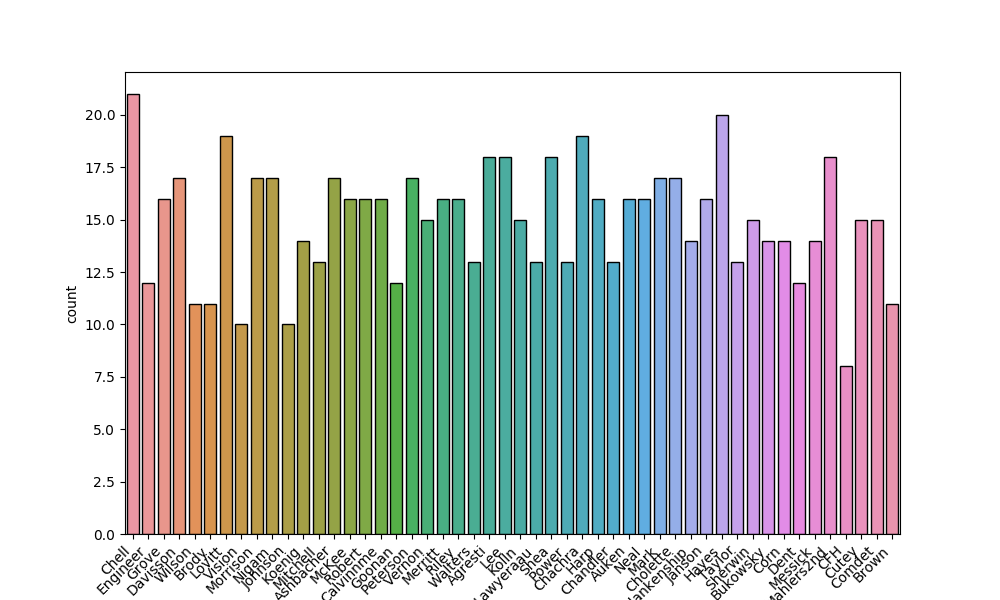
\includegraphics[width=\linewidth]{amazon/plots/target.png}
    \caption{Histogram of the target values}
    \label{fig:amazon-target}
  \end{center}
\end{figure}


\subsection{Feature selection}

We selected features based on SelectKBest, which perform ${\chi}^2$ test to the samples to retrieve the best features. We also used Recursive feature elimination with cross-validation. As seen in Figure \ref{fig:amazon-feature-selection} at least 1000 features should be used to cross the 55 percent mark, however no difference in performance could be detected between 1000 and 4000 selected features.

\begin{figure}[H]
  \begin{center}
    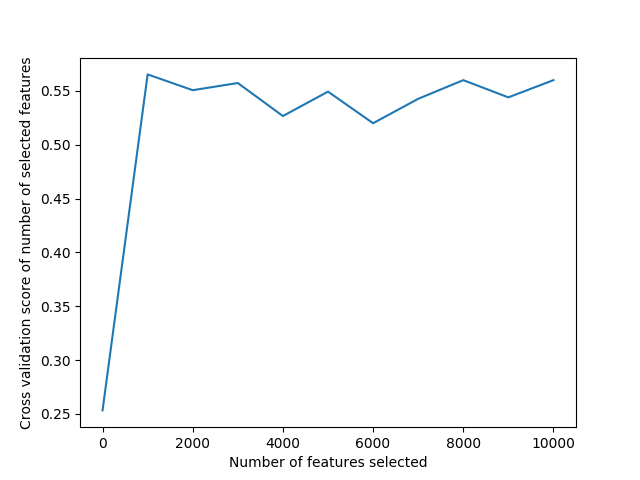
\includegraphics[height=7cm]{amazon/plots/rf_feature_selection.png}
    \caption{Comparison of different metrics}
    \label{fig:amazon-feature-selection}
  \end{center}
\end{figure}

\subsection{K Nearest Neighbors Classifier}

K Nearest Neighbors Classifier worked best with weights set to distance. Meaning that the importance of the k neighbors are weighted by their distance. This increased results by about 10\%. As seen in Figure \ref{fig:amazon-knn-metric-comparison} the manhattan metric worked best.

\begin{figure}[H]
  \begin{center}
    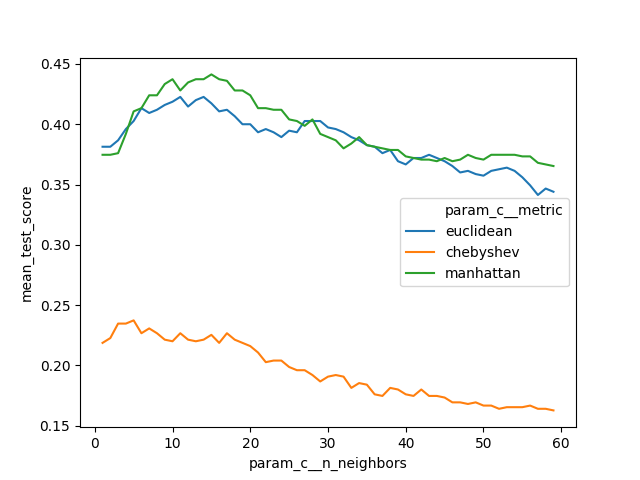
\includegraphics[width=\linewidth]{amazon/plots/knn_metrics.png}
    \caption{Comparison of different metrics}
    \label{fig:amazon-knn-metric-comparison}
  \end{center}
\end{figure}

Preprocessing with MinMax scalar improved results by around 5\% as seen in figure \ref{fig:amazon-knn-comparison}. Scaling with mean and variance did lead to better results, but it was not as good as the min max scaler.

\begin{figure}[H]
  \begin{center}
    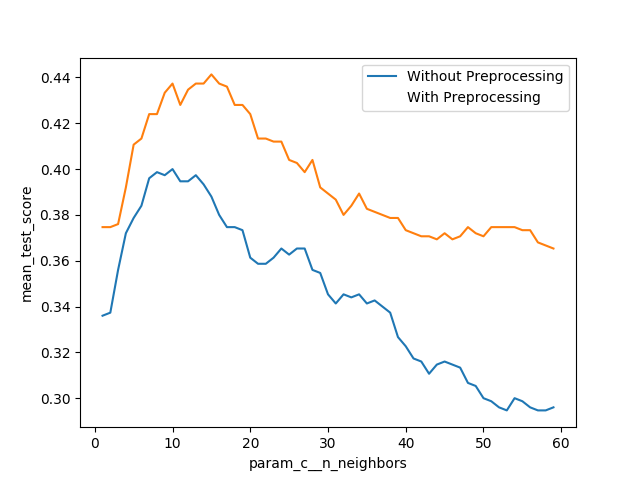
\includegraphics[width=\linewidth]{amazon/plots/knn_comparison.png}
    \caption{Comparison of the best estimators with preprocessing and without preprocessing}
    \label{fig:amazon-knn-comparison}
  \end{center}
\end{figure}


\subsection{Random Forest Classifier}

The best features of Figure \ref{fig:amazon-feature-selection} were used for the Random Forest Classifier. As seen in Figure \ref{fig:amazon-rf-comparison}, a low maximum features yielded good results. We tested different parameters for the minimum samples that lead to splitting and found out that 0.01 works well.

\begin{figure}[H]
  \begin{center}
    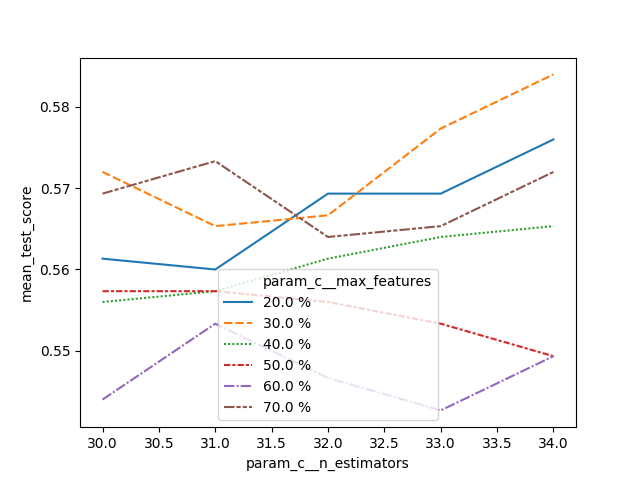
\includegraphics[width=\linewidth]{amazon/plots/rf_comparison.png}
    \caption{Comparison of the best estimators with preprocessing and without preprocessing}
    \label{fig:amazon-rf-comparison}
  \end{center}
\end{figure}

\subsection{Multi-Layer Perceptron Classifier}

Testing out different hyperparamethers for mlp takes quite a lot of time. We were able to get a score of 72 \% accuracy on kaggle by using 2000 selected features with ${\chi}^2$ tests, relu as activation and one hidden layer with 100 neurons. As shown in figure \ref{fig:mlp-comparison} choosing different activation function does not make any difference.

\begin{figure}[H]
  \begin{center}
    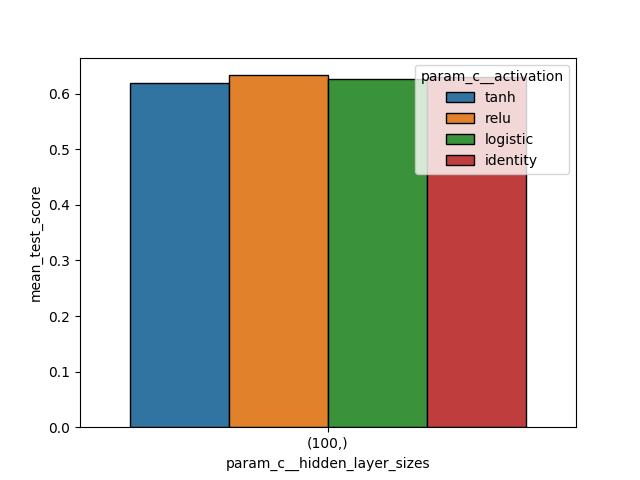
\includegraphics[width=\linewidth]{amazon/plots/mlp_comparison.png}
    \caption{Comparison of the best estimators with preprocessing and without preprocessing}
    \label{fig:mlp-comparison}
  \end{center}
\end{figure}

\subsection{Conclusion}



\begin{table}[H]
\begin{center}
\begin{tabular}{|l|l|l|}
\hline
                       & Preprocessing & No-Preprocessing \\ \hline
KNeighborsClassifier   & 0.4413        & 0.4000           \\ \hline
RandomForestClassifier & 0.6026        & 0.5840           \\ \hline
MLPClassifier          & 0.9666        & 0.9866           \\ \hline
\end{tabular}
\caption{Comparision of accuracy of different techniques with- and without preprocessing}
\end{center}
\end{table}

\begin{table}[H]
\begin{center}
\begin{tabular}{|l|l|l|}
\hline
                       & Holdout & Cross Validation \\ \hline
KNeighborsClassifier   & 0.9333  & 0.9800           \\ \hline
RandomForestClassifier & 0.9666  & 0.9666           \\ \hline
MLPClassifier          & 1.0000  & 0.9866           \\ \hline
\end{tabular}
\caption{Comparision of accuracy of holdout versus cross-validation}
\end{center}
\end{table}

\begin{table}[H]
\begin{center}
\begin{tabular}{|l|l|l|l|l|l|}
\hline
                       & Accuracy & Precision & Recall & F1     & Runtime (sec) \\ \hline
KNeighborsClassifier   & 0.4333   & 0.3847    & 0.4356 & 0.3805 & 30.987        \\ \hline
RandomForestClassifier & 0.9600   & 0.9644    & 0.9600 & 0.9597 & 0.1947        \\ \hline
MLPClassifier          & 0.9800   & 0.9848    & 0.9800 & 0.9793 & 1.5557        \\ \hline
\end{tabular}
\caption{Comparision of different performance metrics and runtimes}
\end{center}
\end{table}



\section{Breast-Cancer Dataset}
The breast cancer dataset was the second mandatory dataset.
We got a score of 97.647\% on kaggle. 
The dataset is is used to classify wheather a tumour is harmful or not.

\subsection{Characteristics}

\begin{itemize}
\item No missing values
\item Binary target class (B and M)
\item Only rational features
\item 30 attributes (disregarding id)
\item 285 samples
\end{itemize}

The attributes contain descriptions of the tumour, for example its radius.

\subsection{Characteristics of Target Value}

A tumour is a cluster of abnormal cells.
If it is a benign tumour it does not contain cancerous cells, whereas a malignant tumour does hold cancerous cells.
Therefore it is more important to correctly classify a sample if it is a malignant tumour than correctly classifying a benign tumour.
It contains two target classes, Benign (B) and Malignant (M).
While 96 of the samples are of type M, 189 are of type B.

\image{breast/plots/countplot.png}{Histogram of the target values}{\label{fig:breast-target}}

% \begin{figure}[H]
%   \begin{center}
%     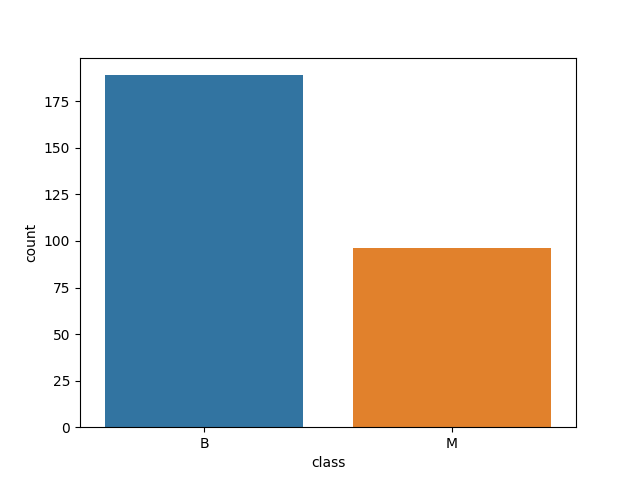
\includegraphics[width=0.8\linewidth]{breast/plots/countplot.png}
%     \caption{Histogram of the target values}
%     \label{fig:breast-target}
%   \end{center}
% \end{figure}

\subsection{Feature Selection}
First, different plots to visualize the data were made.
An example can be seen in Figure \ref{fig:breast-violin}, where it can be observed that the fractalDimensionMean (the feature on the right) is bad for classification while the radiusMean could be more useful as its classes are differently distributed and the mean differs significantly.
Additionally, boxplots were made, which can be observed in Figure \ref{fig:breast-boxplot}.
Boxplots give information about outliers, but the distribution can not be observed as clearly as with violin plots.
Often attributes contain the same information, which can be checked by calculating the correlation of two attributes or graphically interpret their scatter plot as shown in Figure \ref{fig:breast-correlation}.
These plots were analysed and the findings were used afterwards to select the best attributes.


\multimage{breast/plots/violinplot.png}{Violine plot of the first 10 features that were scaled by MinMax}{\label{fig:breast-violin}}{breast/plots/boxplot.png}{Boxplot of the first 10 features that were scaled by MinMax}{\label{fig:breast-boxplot}}

\image{breast/plots/corr_comparision.png}{Scatter plot of two features from the breast cancer dataset}{\label{fig:breast-correlation}}

% \begin{figure}[H]
%   \begin{center}
%     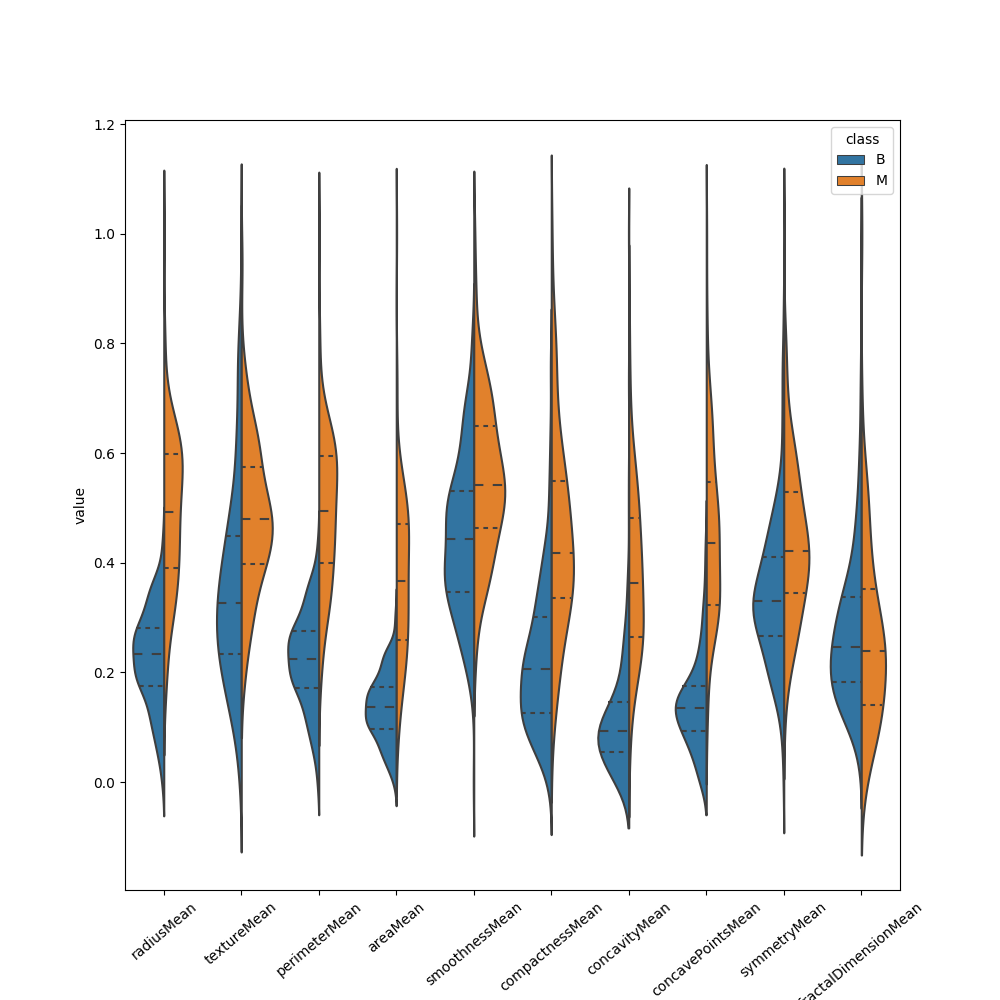
\includegraphics[width=0.8\linewidth]{breast/plots/violinplot.png}
%     \caption{Histogram of the target values}
%     \label{fig:breast-violin}
%   \end{center}
% \end{figure}

Furthermore, recursive feature selection with the Random Forest Classifier was performed as well, which can be observed in Figure \ref{fig:breast-feature-selection}. The results showed that 15 to 30 features work best, which confirms later findings, that feature selection does not necessarily improve performance, since there are only 30 features to select.

\image{breast/plots/rf_feature_selection.png}{Recursive Feature selection}{\label{fig:breast-feature-selection}}

\subsection{K Nearest Neighbors Classifier}

For the K Nearest Neighbour Classifier a grid search with cross validation was used to test different \textit{k}'s from 1 to 30 and different metrics, such as the Euclidean, Chebyshev and Manhattan distance.

As seen in Figure \ref{fig:breast-knn-metrics} Euclidean works best for preprocessed data, whereas Manhattan is better for non preprocessed data.
Concerning the amount of neighbours included in the majority vote, preprocessing works best with a \textit{k} of 10 and weighted distance and non preprocessed with a \textit{k} of 5 and uniform weighted distance.
Comparing the performance of two estimators, preprocessing had a huge impact, which resulted in a 4\% higher accuracy, archiving a performance of 98.6\%.  

Interestingly, Chebychev as a distance metric performs significantly worse compared to the others, especially with a higher \textit{k}.

\image{breast/plots/knn_p_comparision.png}{Comparison of metrics}{\label{fig:breast-knn-metrics}}
% \begin{figure}[H]
%   \begin{center}
%     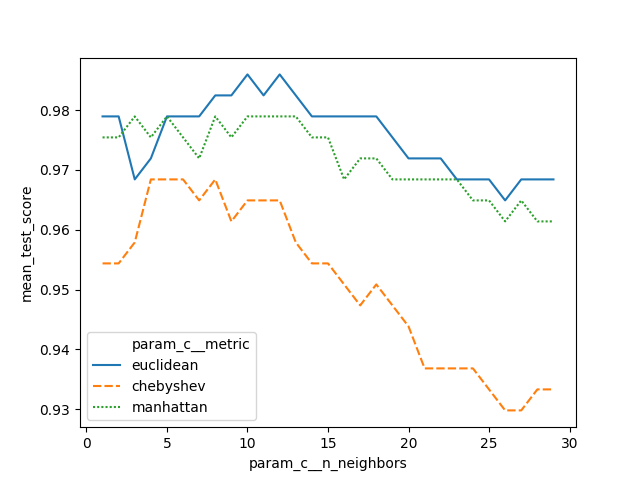
\includegraphics[width=0.8\linewidth]{breast/plots/knn_p_comparision.png}
%     \caption{Histogram of the target values}
%     \label{fig:breast-knn-metrics}
%   \end{center}
% \end{figure}

The previously explained feature selection unfortunately made no improvement, it made the performance even worse, which is shown in the Figure \ref{fig:breast-knn-comparison}.

\image{breast/plots/knn_feature_comparision.png}{Comparison of all Features and selected Features}{\label{fig:breast-knn-comparison}}
% \begin{figure}[H]
%   \begin{center}
%     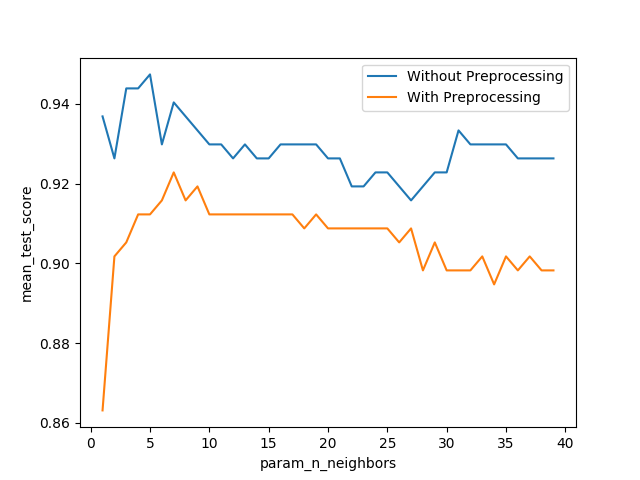
\includegraphics[width=0.8\linewidth]{breast/plots/knn_feature_comparision.png}
%     \caption{Histogram of the target values}
%     \label{fig:breast-knn-comparison}
%   \end{center}
% \end{figure}

\subsection{Random Forest Classifier}

First a randomized search with cross validation was performed to get a first impression for good parameters for the random forest classifier.
It was discovered that the \textit{min\_sample\_split} works best if it is set to 0.04, e.g. the fraction of the minimum samples required to split an internal node is 0.04.
Using the previously obtained information about the parameters, a grid search with cross validation was performed.
It was found that a score of 97.89\% can be obtained by using a maximum of 10\% of the features for an estimator and 47 estimators in total.

\image{breast/plots/rf_np_comparision.png}{Comparison of Random Forest by estimator count and max features}{\label{fig:breast-rf-comparison}}

\subsection{Multi-Layer Perceptron Classifier}

For the Multi-Layer Perceptron Classifier a grid search was performed.
Different layer architectures and activation functions were altered.
As seen in Figure \ref{fig:breast-mlp-comparison}, the best results were obtained with the activation function relu and 3 hidden layers with 30, 15 and 30 neurons.
However the results are mostly the same. However  this is not the case for the Sigmoid or logistic activation function, which is probably due to vanishing gradients.

\image{breast/plots/mlp_p_comparision.png}{comparison of layer sizes and activation functions}{\label{fig:breast-mlp-comparison}}

Preprocessing improved the result as shown in Figure \ref{fig:breast-mlp-np-p-comparison}.
Interestingly the gradients did not vanish for the logistic activation function without preprocessing.

\image{breast/plots/mlp_np_p_comparision.png}{Comparison of activation functions with preprocessing in orange and without preprocessing in blue}{\label{fig:breast-mlp-np-p-comparison}}

\subsection{Conclusion}

Preprocessing leads to better results for all classifiers.
However feature selection leads to worse results.
Therefore the data should only be scaled and all features should be used for classification. Surprisingly, for the breast cancer dataset, K Nearest Neighbours performed better than the MLP in terms of accuracy.

\begin{table}[H]
\begin{center}
\begin{tabular}{|l|l|l|}
\hline
                       & Preprocessing & No-Preprocessing \\ \hline
KNeighborsClassifier   & 0.9862        & 0.9474           \\ \hline
RandomForestClassifier & 0.9789        & 0.9789           \\ \hline
MLPClassifier          & 0.9824        & 0.9614           \\ \hline
\end{tabular}
\caption{Comparison of accuracy of different techniques with- and without preprocessing}
\end{center}
\end{table}

Holdout and cross validation yield similar results.
Therefore holdout can be used for parameter evaluation.

\begin{table}[H]
\begin{center}
\begin{tabular}{|l|l|l|}
\hline
                       & Holdout & Cross Validation \\ \hline
KNeighborsClassifier   & 0.9824  & 0.9862           \\ \hline
RandomForestClassifier & 0.9824  & 0.9789           \\ \hline
MLPClassifier          & 0.9824  & 0.9858           \\ \hline
\end{tabular}
\caption{Comparison of accuracy of holdout versus cross-validation}
\end{center}
\end{table}

The best result was obtained by the K Nearest Neighbours classifier with 98.62\% and the second best by the MLP classifier with 98.58\%.
However on kaggle, KNN only archived a score of 95.29\%, whereas the MLP archived a score of 97.64\%. The reason behind this might be the fact, that on kaggle more training data can be used and this can change the results significantly.
Regarding the runtime KNN classifier is the fastest, followed by the random forest classifier and then the multi layer perceptron, which takes the longest to train.

Concerning the classification of a cancerous tumour cells, it is not an easy task, since wrong prediction can be fatal for the patient.

Therefore, the correct prediction of a malignant as a non cancerous tumour is not that important as the classification of a benign cell. Thus, the best performance metric is the one that minimizes false negatives, which is the case, when using Recall as a performance metric, which also means that KNN is the best classifier in our case for this task, however more samples should be used for a better evaluation, hence a score of 98.58\% is still not sufficient.

\begin{table}[H]
\begin{center}
\begin{tabular}{|l|l|l|l|l|l|}
\hline
                       & Accuracy & Precision & Recall & F1     & Runtime (sec) \\ \hline
KNeighborsClassifier   & 0.9862   & 0.9902    & 0.9800 & 0.9841 & 0.0016        \\ \hline
RandomForestClassifier & 0.9756   & 0.9752    & 0.9715 & 0.9726 & 0.0677        \\ \hline
MLPClassifier          & 0.9858   & 0.9902    & 0.9783 & 0.9831 & 0.8999        \\ \hline
\end{tabular}
\caption{Comparison of different performance metrics and runtimes}
\end{center}
\end{table}



\section{Iris Dataset}
\subsection{Characteristics}

\subsection{Characteristics of Classifiers}

\subsection{K Nearest Neighbors}

\subsection{Decision Trees}

\subsection{Multi-Layer Perceptron}

\section{Online-Shoppers-Intention}


The Online Shoppers Purchasing Prediction dataset fits somewhere in between the others as it has a low to medium amount of features and its sample size is on the medium to high spectrum. It also complements the Breast Cancer dataset as it is also a binary classification task. Another reason why  this dataset has been chosen, is that is a lot closer to real world applications than some other posed Machine Learning questions. From a entrepreneurial standpoint it is very interesting for business processes as it can aid in ameliorating other internal processes. With it one can facilitate answering questions such as ''Will this person buy something?'' and ''How can we change our internal processes, based on the important attributes we identified, to increase the percentage of people buying things?''. We first take a general look on the different attributes and try to find the most important features by analysing the data. Afterwards we try out the above mentioned classifiers with a few different parameters to find the right settings based on this dataset. A final summary will be given by comparing the best parameters in combination with Preprocessing vs No-Preprocessing, Holdout vs Cross Validation and taking a look at a few different performance metrics. 

\subsection{Characteristics}

\begin{itemize}
\item Missing values in the original dataset
\item Binary Target Class Revenue
\item 18 attributes (10 numerical, 8 categorical)
\item Nominal attributes (Browser, OS, Region, ...)
\item Interval attributes (Bounce Rate, Exit Rate, ...)
\item Ratio attributes (Informational Duration, ProductRelated Duration, ..)
\item 12330 samples
\end{itemize}

\subsection{General Preprocessing} \label{GenPrepro}
The \textbf{original} dataset contained 14 missing values which could easily be resolved by just removing the affected rows. Another thing that could be done, would be to replace the ratio and interval attributes with the mean and the ordinal and the categorical attributes with the median. On the UCI Machine Learning Repository we were able to find a version of this dataset which contained no missing values, hence no further action was needed. \\
\newline
As there are 8 categorical values these need to be encoded to be available for our Classifiers. Instead of using Label Encoding, where higher values could be biased, we used One Hot Encoding. This added about 40 features to our already existing ones.

\subsection{Characteristics of Target Value}
While accuracy is a great measure for classification problems when one has symmetric datasets (amount of false positves and false negatives is approximately the same), it is not optimal for our model.
As can be seen in \secref{fig:rev_box} only 15.5\% (1908) were positive class samples that ended with shopping and the rest (10422) did not end with shopping. It is more important to not falsely identify Buyers as Non-Buyers. For example we would rather focus on more people than necessary instead of potentially losing profit and customers. Due to this we chose Recall as our primary performance metric when optimizing the different Classifiers as there is a high cost of False Negatives and our data is skewed.
\image{onlineshop/plots/revenue_boxplot.png}{Target Class Distribution}{\label{fig:rev_box}}

\subsection{Feature Selection}
% Heatmap Correlation
Now having 57 attributes, it is important to remove features and thus random noise which could lead to overfitting to the training data. Reducing the dimensions also allows us to reduce training time and thus lets us train with more different parameters. Looking at the correlation matrix in \secref{fig:heat} one can see features that are correlated such as PageValues, ExitRates, ProductRelated,ProductRelated Duration BounceRates, etc.  
\image{onlineshop/plots/heatmap.png}{Heatmap of the different attributes of the Online Shopping Prediction dataset}{\label{fig:heat}} \\
\newline
Using Scikitlearn's SelectKBest and RandomForestClassifier we analysed the features, correlating with the Revenue target, more in depth. \\
\newline

The top 10 correlated features, with their respective scores, found through SelectKBest are as follows:

\begin{figure}
\begin{floatrow}
\ffigbox[\FBwidth][][]{\caption{Top 10 features selected by RandomForestClassifier}}
    {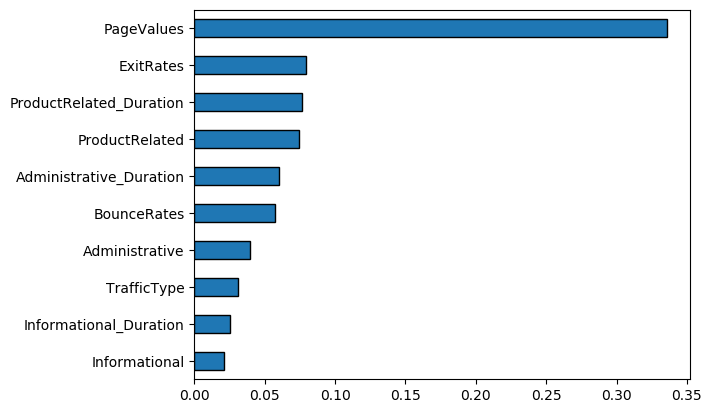
\includegraphics[width=8cm]{onlineshop/plots/feature_selection_random_forest_classifier.png}}

\capbtabbox{%
  \begin{tabular}{l|r}
Atribute                  & \multicolumn{1}{l}{Score} \\ \hline
ProductRelated\_Duration  & 877404.34                 \\
PageValues                & 175126.81                 \\
Administrative\_Duration  & 41754.84                  \\
Informational\_Duration   & 35059.78                  \\
ProductRelated            & 19317.29                  \\
Administrative            & 1133.97                   \\
Informational             & 357.98                    \\
Month\_Nov                & 223.55                    \\
VisitorType\_New\_Visitor & 115.34                    \\
Month\_May                & 55.00                     \\
SpecialDay                & 53.80                     \\
OperatingSystems\_3       & 48.55                    
\end{tabular}
}{%
  \caption{Top 10 features selected by SelectKBest}%
}
\end{floatrow}
\end{figure}

Looking at both models one can see that the two most important attributes are 'ProductRelated\_Duration' and 'PageValues.
Using the information from the two selections and through trial and error, by playing around with a few different attribute combinations, we have found the following top attributes:

\begin{itemize}
    \item Top 3: ['ProductRelated\_Duration', 'PageValues', 'Administrative\_Duration']
    \item Top 7: Top 3 + ['Informational\_Duration',  'ProductRelated', 'Administrative', 'Informational']
    \item Top 12: Top 7 +  ['BounceRates', 'ExitRates', 'PageValues', 'Month\_Nov', 'TrafficType' ]      
\end{itemize}
Performance comparisons between the different Top attributes lists can be found in the following sections.  



\subsection{K Nearest Neighbours Classifier}
Looking at \secref{fig:knn_wo_pre} one can see that using the most attributes leads to the best performance.  Interesting to note here, is that the best recall values were achieved when using k = 1 and thus only looking at the closest neighbour. 

\begin{figure}
\begin{floatrow}
\ffigbox[\FBwidth][][]{\caption{Without Scaling (metric: Manhattan, weights: Uniform)}}
    {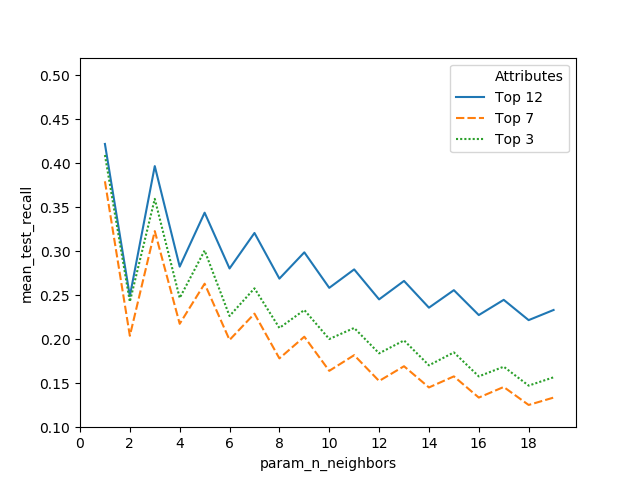
\includegraphics[width=6cm]{onlineshop/plots/knn_wo_preprocessing.png}\label{fig:knn_wo_pre}}
\ffigbox[\FBwidth][][]{\caption{With MinMax Scaling (metric: Uniform, Top 12 Attributes)}}
    {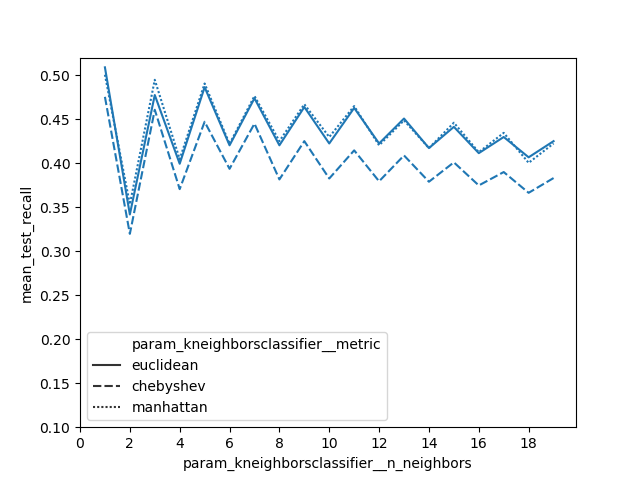
\includegraphics[width=6cm]{onlineshop/plots/knn_uniform_metric_comparison.png}\label{fig:knn_w_pre}}
\end{floatrow}
\end{figure}

As can be seen in \secref{fig:knn_w_pre} scaling the data leads to a best case improvement of around 0.07 compared to the unscaled data which only increases with increasing k. Another thing that scaling the data does, is reducing the overall decrease of the recall with changing k. This figure also shows that the euclidean and manhattan metric perform very similar for this dataset while the chebyshev performs slightly worse. \\
\newline
A general analysis beforehand showed that, while different weight parameters change how the recall values react to different k's, with \textit{uniform} being more sensitive compared to  \textit{distance}, they do not change the best achievable values.
\subsection{Random Forest Classifier}
For Random Forest Classifier we have used GridSearchCV to try out a few different parameters like \textit{n\_estimators, max\_depth and the criterion}. \\
\newline
By doing a few pre tests and comparing how the criterion affects the recall value, we note that they lead to very similar results for this dataset. Since Gini is a tiny bit better than Entropy, it will be used for the other comparisons. \\
\newline

\begin{figure}
\begin{floatrow}
\ffigbox[\FBwidth][][]{\caption{Comparison of \textit{n\_estimators} for different \textit{max\_depth} values}}
    {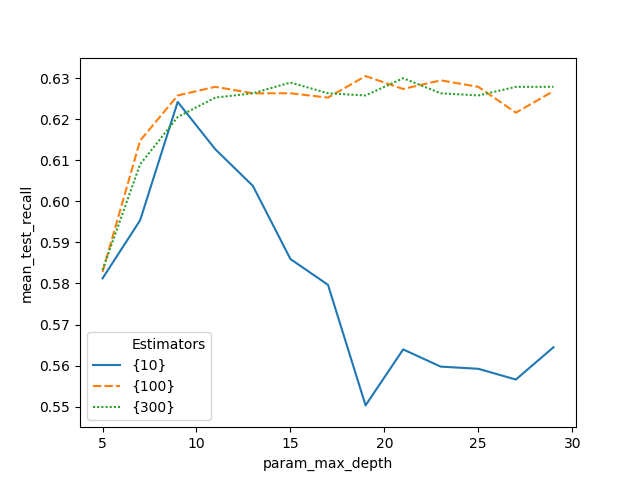
\includegraphics[width=6cm]{onlineshop/plots/rfc_n_estimators_comparison.png}\label{fig:rf_n_estim}}
\ffigbox[\FBwidth][][]{\caption{Scaling vs No Scaling comparison (100 Trees)}}
    {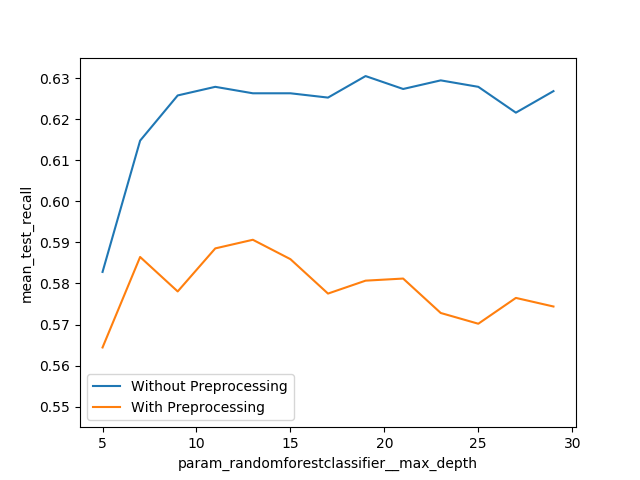
\includegraphics[width=6cm]{onlineshop/plots/rfc_preprocessing_comparison.png}\label{fig:rfc_pre}}
\end{floatrow}
\end{figure}

Looking at the different n\_estimators in \secref{fig:rf_n_estim} we can see that a higher n\_estimators makes up for the overfitting which will be achieved by having a too high max\_depth value. This makes sense as the amount of trees within a forest is a good way to control overfitting. On the other hand after a certain point it makes no difference if there are 100 or 300 trees. \\
\newline
As trees are very robust and thus do not need Preprocessing most of the time, applying a MinMaxScaler to our data actually led to worse values which is visualized in \secref{fig:rfc_pre}.

\subsection{Multi-Layer Perceptron Classifier}
Finally, taking a look at the more sophisticated Multi-Layer Perceptron, we have tried out a few different parameter settings, firstly manually configuring them and then iterating over a few different combinations with GridSearch. The paremeters we have looked at were: hidden layer sizes (layer and neuron amount), activation functions, different solvers, learning rate and the alpha penalty regularization parameter.


\begin{figure}
\begin{floatrow}
\ffigbox[\FBwidth][][]{\caption{Comparison of different \textit{hidden\_layer\_sizes} with stochastic gradient descent optimizer}}
    {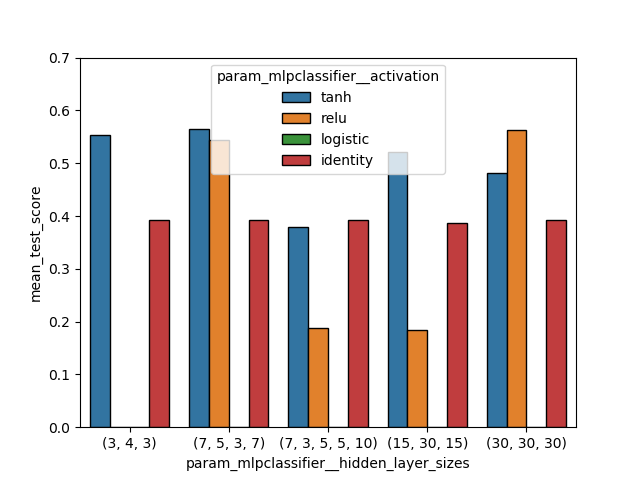
\includegraphics[width=6cm]{onlineshop/plots/mlp_solver_comparisonsgd.png}\label{fig:mlp_sgd}}
\ffigbox[\FBwidth][][]{\caption{Comparison of different \textit{hidden\_layer\_sizes} with adam optimizer}}
    {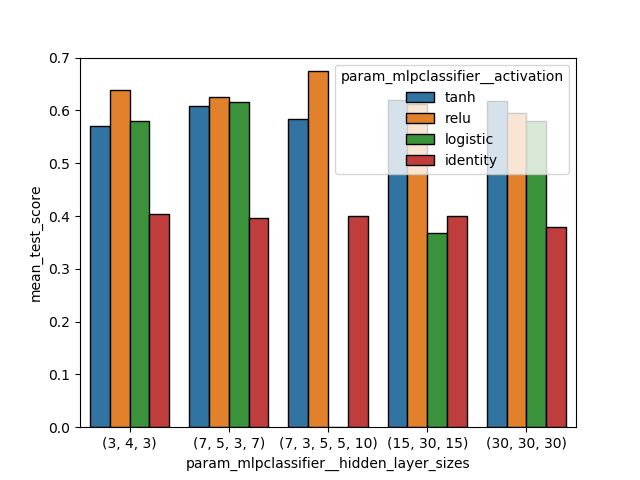
\includegraphics[width=6cm]{onlineshop/plots/mlp_solver_comparisonadam.png}\label{fig:mlp_adam}}
\end{floatrow}
\end{figure}
As can be seen in \secref{fig:mlp_sgd}, using the wrong weight optimizer (stochastic gradient descent in this case) leads to much worse recall scores, with some of them even being zero (no True Positives predicted). Using the stochastic gradient descent version adam (by Kingma, Diederik, and Jimmy Ba) we were able to achieve much better and more consistent scores.

On the other hand the difference between having a constant learning rate of 0.001 and an adaptive one (divide learning rate by 5 if the training loss does not decrease for 2 consecutive epochs) was negligible, with the adaptive one being only 0.02 better in the best case. The same goes for different alpha values. \\
\newline
What can be observed is that using tangens hyperbolicus and Relu provides far better results no matter the layer sizes. The identity function performed much worse, achieving only a recall score of around 0.4 while the others were able to achieve scores of above 0.6 for at least one parameter setting. On the other hand, while the logistic activation function even was able to achieve a better score than the tangens hyperbolicus (hidden layer sizes (3,4,3)), it performed much worse in a few settings (hidden layer sizes (7, 3, 5, 5, 10) or (15, 30, 15)) whereas the others stayed consistent. \\
\newline
It can be said, that while the hidden layer sizes obviously matter, the activation function played a much bigger role for getting the best values. On average for this dataset relu performed the best, followed by tangens hyperbolicus with logistic and identity performing the worst. The best result (0.6750 recall) was achieved when using more layers and relu as the activation function. The amount of neurons seemed to not make too much of a difference.


\subsection{Conclusion}
\subsubsection{Preprocessing vs No-Preprocessing}
To be able to look at more than just the numerical values, \textit{No-Preprocessing} in this case stands for the data after the general Preprocessing (One Hot Encoding, remove Missing values, ...), mentioned in \secref{GenPrepro}, has been done. We compare the unpreprocessed data with the data after MinMax scaling.\\% and after introducing a new feature by weighting the outliers.
\newline
Analysing \secref{tab:onl_pre_no_pre}, we can see that using a MinMax Scalar only works for the K Nearest Neighbors Classifier and the Multi-Layer Perceptron. As the Random Forest Classifier does not work with distances,  the ranges of the different attributes does not matter. Hence using a MinMaxScaler actually leads to worse results for the Random Forest Classifier.

% TODO

\begin{table}[h]
\begin{center}
\begin{tabular}{|l|l|l|}
\hline
                       & Preprocessing & No-Preprocessing \\ \hline
KNeighborsClassifier   & \textbf{0.5089}        & 0.4219          \\ \hline
RandomForestClassifier & 0.5906        & \textbf{0.6305}           \\ \hline
MLPClassifier          & \textbf{0.6750}        & 0.6106           \\ \hline
\end{tabular}
\caption{Recall comparison with- and without MinMax Scaling}
\label{tab:onl_pre_no_pre}
\end{center}
\end{table}

\subsubsection{Holdout vs Cross Validation}
The cross validation results are the best ones achieved during the GridSearch parameter iteration, hence they are the same ones as the ones as in the table of the previous section (Preprocessing values for KNeighborsClassifier and MLPClassifier, No-Preprocessing for RandomForestClassifier). To calculate the Holdout score we used the best\_estimator of the respective Classifier and then fit the data on that estimator. 
By comparing the achieved holdout and cross validation values we can see that the holdout method sometimes leads to better results and sometimes to worse. This is a possibility since the training split is randomly chosen, which plays a big part in how the data will be tested. In these particular cases Holdout led to only marginally better results for KNeighborsClassifier and RandomForestClassifier, while MLPClassifier was a lot better while using Cross Validation. 

\begin{table}[h]
\begin{center}
\begin{tabular}{|l|l|l|}
\hline
                       & Holdout & Cross Validation \\ \hline
KNeighborsClassifier   & \textbf{0.5236}  & 0.5089           \\ \hline
RandomForestClassifier & \textbf{0.5863}  & 0.5817           \\ \hline
MLPClassifier          & 0.5681  & \textbf{0.6750}           \\ \hline
\end{tabular}
\caption{Comparison of accuracy of holdout versus cross-validation}
\end{center}
\end{table}

%
\subsubsection{Different Performance Metrics}
To analyse how the different classifiers compare for this dataset we have tried to optimize the models in regards to recall as mentioned above. Using GridSearchCV's best\_estimator we were able to find the optimal parameter settings, which were as follows (if parameters are undefined, the default ones for the respective sklearn models were chosen):
\begin{itemize}
    \item K Neigbors Classifier: MinMax Scaling, leaf\_size=30, n\_neighbors=1, metric='euclidean', 
    \item Random Forest Classifier: No Scaling, criterion='gini', max\_depth=19, max\_features='auto', n\_estimators=100
    \item MLP Classifier: MinMax Scaling, activation='relu', alpha=0.001,\\learning\_rate='adaptive',
    learning\_rate\_init=0.001, max\_iter=3000, \\ hidden\_layer\_sizes=(7, 3, 5, 5, 10) (some parameters may change due to randomness)
\end{itemize}

\begin{table}[h]
\begin{center}
\begin{tabular}{|l|l|l|l|l|l|}
\hline
                       & Accuracy & Precision & Recall & F1     & Runtime (sec) \\ \hline
KNeighborsClassifier   & 0.8525   & 0.5483  & 0.5089 & 0.5213 & \textbf{0.0434}        \\ \hline
RandomForestClassifier & \textbf{0.8982}   &\textbf{0.7187}    & 0.5817   & \textbf{0.6408}   & 1.0573        \\ \hline
MLPClassifier          & 0.8914   & 0.6648    & \textbf{0.6152}   & 0.6375   & 5.3267        \\ \hline
\end{tabular}
\caption{Comparison of different performance metrics and runtimes}
\label{tab:onl_summ}
\end{center}
\end{table}

Analysing the table in regards to Accuracy, we see that the different classifiers all perform very similarly, with K Neighbors Classifier being around 4 percent worse than the others. This is to be expected since our data is quite skewed, only having around 15.5\% positive target values. Due to this it is especially important to look at the other performance metrics. \\
\newline
While RandomForest Classifier only is marginally better than MLP Classifier in regards to accuracy, it achieves a precision score of around 72 percent which is more than 5 percent better than the one achieved by MLP and more than 5 percent better than the one achieved by K Neighbors. \\
\newline 
Using GridSearchCV to optimize our model in regards to recall, we were able to achieve a recall score of around 62 percent with the MLP Classifier and a score of 58 percent with the Random Forest Classifier. Looking at the F1 score we can see that Random Forest Classifier and MLP Classifier perform very similarly, both achieving a worthy score of around 0.64.\\
\newline
Concering runtime we can see that the K Neighbors Classifier obviously performs best as it is a lazy learner and does not need any pre fitting. With increasing complexity, the runtime also increases which is why the MLP Classifier took over a hundred times longer to fit than the K Neighbors Classifier and over 5 times longer than the Random Forest Classifier.\\
\newline
To answer the question, which Classifier performs best for this dataset, we need to differentiate a few different scenarios.
If we only care about the accuracy score and need to get results fast, the best option would be the K Neighbors Classifier as it performs a lot better in regards to runtime and is comparable in terms of accuracy.\\
Comparing the Random Forest Classifier and the MLP Classifier we can see that there is a draw in terms of Accuracy and F1 since the differences between the two classifiers are negligible. If we say that a high precision, i.e. there is a higher cost of falsely identifying Positives, and a faster runtime are more important, then the Random Forest Classifier would be the best choice.\\
Since we defined that recall is our most important metric (the opportunity costs of passing up on a buying candidate are high) the MLP Classifier is the best one for this particular dataset.

\newpage
\section{Overall Conclusion}
In this section we will analyse how useful the chosen classifiers are in regards to our specific datasets and how they compare to each other. \\
\newline
First of all it needs to be mentioned that the specific datasets pose different classification tasks as we have got 2 binary classifications (Online Shopping Predictions, Breast Cancer) and 2 Multiclass classifications (Iris, Amazon). Thus a direct comparison must be taken with a grain of salt, as having multiple classes adds another layer of complexity. 

Interesting to note here is that even the least sophisticated classifier, K Neighbors, was able to achieve 98 percent in every above mentioned performance metric for the Iris and Breast Cancer dataset. As seen in the previous plots, this can be explained by the good distinguishability of the specific features and allows the k Neighbors algorithm to look at the closest datapoints which are in the same baskets/classes. 
Comparing K Neighbors  to the Random Forest Classifier, we see that more complexity does not have to lead to better results. For these 2 datasets the Random Forest Classifier actually performed marginally worse for every metric and on top of that took a lot longer relatively to fit. The Random Forest Classifier still is a good model as it performed very similar to K neighbors for these datasets. For the more complex datasets (Online Shopping Predictions, Amazon) it achieved much better scores than the K Neighbors Classifier and even had the highest accuracy and precision score for the Online Shopping Predictions dataset. \\
\newline
A slight trend/observation can be made out for the different classifiers: 
\begin{itemize}
    \item The K Neighbors Classifier performs best for simpler datasets where the features are more distinguishable.
    \item Random Forest and MLP Classifier seem to perform well for simple and more complex datasets.
    \item The MLP Classifier performs better than the others when the underlying structure to be learned is more sophisticated.
\end{itemize} 
Concerning the question about which classifiers prove useful, one needs to define a threshold for when we say that a model is applicable for real world use. For the Iris and Breast Cancer dataset the choice of classifier does not make too much difference, especially considering the fact that we only have a few datapoints and a few more could skew the scores for one classifier or the other. \\
For the Online Shopping Predictions one could say that the Random Forest Classifier's results are good enough if one is only interested in the accuracy and the precision score. This could be the case if we say that the cost of false positives is high, for example if we'd send out expensive gifts for every potential buyer. Considering the fact that this model will most likely be used to do some form of marketing it is more plausible that we care more about the cost of false negatives, i.e. potentially losing customers. Thus for the Online Shopping Predictions dataset either a Random Forest or a MLP Classifier could be applicable if one deems the achieved scores acceptable. \\
Regarding the Amazon dataset it is clear that the MLP Classifier performs best at it achieves scores which are 10 percent higher (for every metric) than the Random Forest Classifier and takes less than a fifth of the time to fit.
\newline
% allgemein Parameter TODO
Are the Classifiers Sensitive to parameter changes? 
We have found that generally a higher amount of n\_estimators, i.e. trees, leads to a better performance. This can be explained by the fact that many trees help to create an average which does not overfit to certain scenarios.


%TODO Preprocessing vs No-Preprocessing General Tabelle
Comparing the effects of Preprocessing, we see that the K Neighbors and MLP Classifier seemed to generally benefit the most from Scaling (excluding Iris since it only has a few features) while it did not have too much of of an impact on the Random Forest Classifier and even lead to a worse score for the Online Shopping Predictions dataset.

Another thing to keep in mind is that 

While the amount of samples played a big role in the runtimes of the different classifiers, the amount of selected features had the biggest impact. Obviously the number of samples affects how long/often the model needs to be trained and updated (MLP), but the number of features affect how long it takes to calculate the comparisons to the other datasets and how long one update cycle is.

% increasing the amount of samples by a factor of 100 lead to a runtime increase of ... . Adding onto that going from ~10 features to over a thousand increased the runtimes of around ...

\begin{table}
\begin{center}
\begin{adjustwidth}{-4cm}{-4cm}  
\begin{tabular}{|l|ccccr|ccccr|ccccr|}
\hline
                                                                      & \multicolumn{5}{c|}{K Neighbors} & \multicolumn{5}{c|}{Random Forest} & \multicolumn{5}{c|}{MLP} \\ %\hline
                                                                      & A    & P    & R    & F1    & sec   & A     & P    & R    & F1    & sec    & A   & P  & R  & F1  & sec  \\ \hline
Iris                                                                  & 0.98   & 0.98  & 0.98 & 0.98 & 0.0014 & 0.96   & 0.96    & 0.96 & 0.96 & 0.0695 & 0.98   & 0.98    & 0.98 & 0.98 & 0.7719   \\ \hline
\begin{tabular}[c]{@{}l@{}}Online Shopping\\ Predictions\end{tabular} & 0.85   & 0.55  & 0.51 & 0.52 & 0.0434 & 0.90   & 0.72    & 0.58   & 0.64   & 1.0573 & 0.89   & 0.66    & 0.62   & 0.64   & 5.3267   \\ \hline
Breast Cancer                                                         & 0.99   & 0.99    & 0.98 & 0.98 & 0.0016     & 0.98   & 0.98    & 0.97 & 0.97 & 0.0677      & 0.99   & 0.99    & 0.99 & 0.98 & 0.8999    \\ \hline
Amazon                                                                & 0.43 & 0.38 & 0.44 & 0.38 & 30.9870  & 0.59 & 0.54 & 0.59 & 0.54 & 481.1520 &  0.70 & 0.66 & 0.69 & 0.65 & 87.9900     \\ \hline
\end{tabular}
\end{adjustwidth}
\end{center}
\end{table}


% _________________________OVERALL CONCLUSION____________________________________________
\section{Overall Conclusion}
In this section we will summarize and analyse how useful the chosen classifiers are in regards to our specific datasets and how they compare to each other. \\
\newline
First of all it needs to be mentioned that the specific datasets pose different classification tasks as we have got 2 binary classifications (Online Shopping Predictions, Breast Cancer) and 2 Multiclass classifications (Iris, Amazon). Thus a direct comparison must be taken with a grain of salt, as having multiple classes adds another layer of complexity. \\
\newline
Looking at \secref{tab:summ} it is interesting to note that even the least sophisticated classifier, K Neighbors, was able to achieve 98 percent in every above mentioned performance metric for the Iris and Breast Cancer dataset. As seen in the previous plots, this can be explained by the good distinguishability of the specific features and allows the k Neighbors algorithm to look at the closest datapoints which are in the same baskets/classes. \\
Comparing K Neighbors  to the Random Forest Classifier, we see that more complexity does not have to lead to better results. For these 2 datasets the Random Forest Classifier actually performed marginally worse for every metric and on top of that took a lot longer relatively to fit. The Random Forest Classifier still is a good model as it performed very similar to K neighbors for these datasets. For the more complex datasets (Online Shopping Predictions, Amazon) it achieved much better scores than the K Neighbors Classifier and even had the highest accuracy and precision score for the Online Shopping Predictions dataset. \\
\newline
A slight trend/observation can be made out for the different classifiers: 
\begin{itemize}
    \item The K Neighbors Classifier performs well for simpler datasets, where the features are more distinguishable.
    \item Random Forest and MLP Classifier seem to perform well for simple and more complex datasets.
    \item The MLP Classifier performs better than the others when the underlying structure to be learned is more sophisticated.
\end{itemize} 
Concerning the question about which classifiers prove useful, one needs to define a threshold for when we say that a model is applicable for real world use. For the Iris and Breast Cancer dataset the choice of classifier does not make too much of a difference, especially considering the fact that we only have a few datapoints and a few more could skew the scores for one classifier or the other. \\
For the Online Shopping Predictions one could say that the Random Forest Classifier's results are good enough if one is only interested in the accuracy and the precision score. This could be the case if we say that the cost of false positives is high, for example if we'd send out expensive gifts for every potential buyer. Considering the fact that this model will most likely be used to do some form of marketing it is more plausible that we care more about the cost of false negatives, i.e. potentially losing customers. Thus for the Online Shopping Predictions dataset either a Random Forest or, more likely, the MLP Classifier could be applicable if one deems the achieved scores acceptable. \\
Regarding the Amazon dataset it is clear that the MLP Classifier performs best at it achieves scores which are 10 percent higher (for every metric) than the Random Forest Classifier and takes less than a fifth of the time to fit. Nevertheless, as even the best classifiers for Online Shopping Predictions and the Amazon dataset do not seem to have non substential error rates, one needs to take the model's real world applicability with a grain of salt. \\
\newline

\begin{table}
\begin{adjustwidth}{-3.0cm}{-3.0cm}  
\begin{center}
\begin{tabular}{|l|ccccr|ccccr|ccccr|}
\hline
                                                                      & \multicolumn{5}{c|}{K Neighbors} & \multicolumn{5}{c|}{Random Forest} & \multicolumn{5}{c|}{MLP} \\ %\hline
                                                                      & A    & P    & R    & F1    & sec   & A     & P    & R    & F1    & sec    & A   & P  & R  & F1  & sec  \\ \hline
Iris                                                                  & 0.98   & 0.98  & 0.98 & 0.98 & 0.0014 & 0.96   & 0.96    & 0.96 & 0.96 & 0.0695 & 0.98   & 0.98    & 0.98 & 0.98 & 0.7719   \\ \hline
\begin{tabular}[c]{@{}l@{}}Online Shopping\\ Predictions\end{tabular} & 0.85   & 0.55  & 0.51 & 0.52 & 0.0434 & 0.90   & 0.72    & 0.58   & 0.64   & 1.0573 & 0.89   & 0.66    & 0.62   & 0.64   & 5.3267   \\ \hline
Breast Cancer                                                         & 0.99   & 0.99    & 0.98 & 0.98 & 0.0016     & 0.98   & 0.98    & 0.97 & 0.97 & 0.0677      & 0.99   & 0.99    & 0.99 & 0.98 & 0.8999    \\ \hline
Amazon                                                                & 0.43 & 0.38 & 0.44 & 0.38 & 30.9870  & 0.59 & 0.54 & 0.59 & 0.54 & 481.1520 &  0.70 & 0.66 & 0.69 & 0.65 & 87.9900     \\ \hline
\end{tabular}
\caption{Performance Metrics and Runtime Summary} 
\label{tab:summ}
\end{center}
\end{adjustwidth}
\end{table}
\subsection{Parameter Sensitivity}
Analysing the sensitivity of the classifiers in regards to parameter changes, we have found that simply changing one parameter sometimes could completely turn the result into another direction. This was especially observable for the MLP Classifier where simply choosing adam as the optimizer instead of the regular stochastic gradient descent turned a recall score from 0.2 to 0.675 (see \secref{fig:mlp_sgd} and \secref{fig:mlp_adam}). On top of that the MLP was very sensitive in regards to the activation function with tangens hyperbolicus generally providing the best results and the logistic activation function generally performing the worst.\\
We have found that a higher amount of n\_estimators, i.e. trees, usually leads to a better performance up to a certain point. This can be explained by the fact that many trees help to create an average which does not overfit to certain scenarios.\\
In regards to K Neighbors we have seen that we tend to get the best results with Euclidean and Manhattan as the distance metric.  
Another thing that could be observed for the K Neighbors Classifier, was that preprocessing the data in general also lead to an increase of k, since with the scaled ranges  more datapoints could now be considered. \\
\newline
%TODO Preprocessing vs No-Preprocessing General Tabelle
\subsection{Preprocessing Effects}
Comparing the effects of Preprocessing, we see that the K Neighbors and MLP Classifier seemed to generally benefit the most from Scaling (excluding Iris since it only has a few features) while it did not have too much of of an impact on the Random Forest Classifier and even lead to a worse score for the Online Shopping Predictions dataset. For the Iris dataset, preprocessing lead to a decrease in performance for the K Neighbors Classifier and the MLP Classifier.

\subsection{Runtime}
While the amount of samples played a big role in the runtimes of the different classifiers, the amount of selected features had the biggest impact. Obviously the number of samples affects how long/often the model needs to be trained and updated (MLP), but the number of features affect how long it takes to calculate the comparisons to the other datasets and how long one 'calculation cycle' is. Iris and Breast Cancer which contained a similar amount of samples/features and also had very similar scores also seemed to  have pretty much the exact same fitting times. Increasing the samplesize to around 12.000 (Online Shopping with around 40 times more samples than Breast Cancer's 300) led to a runtime increase by a factor of 30 for K Neighbors, 15 for Random Forest and 5 for MLP.\\ On the other hand increasing the feature amount by a factor of 100 (we selected over a thousand features for the Amazon dataset and only around 15 for Breast Cancer) we saw a runtime increase by a factor of 20.000 for K Neighbors, 7.000 for Random Forest and 100 for MLP (MLP: less features or else it would take too long). 
Comparing the high number of samples of the Online Shopping Predictions Dataset with the high number of features of the Amazon dataset runtime ratios of 700, 450 and 20 can be noted. Thus it seems that the runtime of K Neighbors seemed to be affected the most by an increase of samples/features, followed by Random Forest and then MLP. \\
\newline
Except for the Amazon dataset, where we achieved the best results with only a high amount of features, the MLP took around $c*10^1$ times longer to fit than the Random Forest Classifier and around $c* 10^2$ times longer than the K Neighbors Classifier.\\
Observing the Amazon Dataset we see that the ratio of $c*10^1$ seems to hold true if we compare Random Forest to K Neighbors Classifier. The runtime ratio MLP to Random Forest did not scale as it did for the other datasets and MLP was even faster than Random Forest, which could be explained by the parameter choice in the best case scenarios. \\
Another thing to keep in mind is that the parameters have got a huge influence on the runtimes. Increasing the amount of neighbors/amount of trees \& max depths/amount of iterations \& neurons for the respective classifiers also lead to an increase in runtimes.
\end{document}
